\documentclass[parskip=full]{scrartcl}

\usepackage{amsmath}
\usepackage{hyperref}
\usepackage{graphicx}
\graphicspath {{images/}}
\hypersetup{
    colorlinks=true,
    citecolor=blue
}

\renewcommand\thesubsection{\thesection.\alph{subsection}}


\begin{document}


\title{CS698 - Assignment 3}
\subtitle{Winter 2017}
\author{
    Vineet John\\
    \texttt{v2john@uwaterloo.ca}
}
\date{\today}
\maketitle


\section{Gaussian Kernel Derivation} % (fold)
\label{sec:gaussian_kernel_derivation}

    \subsection*{Objective} % (fold)
    \label{sub:objective_1}
        Prove that the Gaussian kernel can be expressed as the inner product on an infinite dimensional feature space
        \begin{equation} \label{eqn:objective}
            k(x, x\prime) = e^{\frac{- {\lVert x - x\prime \rVert}^2}{2\sigma^2}}
        \end{equation}

    % subsection objective_1 (end)

    \subsection*{Proof} % (fold)
    \label{sub:proof_1}

        Expanding the exponent term in equation \ref{eqn:objective}, we get
        $$k(x, x\prime) = e^{\frac{-(x^Tx - 2x^Tx\prime + x\prime^Tx\prime)}{2\sigma^2}}$$

        Separating the exponent terms
        $$k(x, x\prime) = e^{\frac{-x^Tx}{2\sigma^2}} e^{\frac{x^Tx\prime}{\sigma^2}} e^{\frac{- x\prime^Tx\prime)}{2\sigma^2}}$$

        which can be written in general terms as
        \begin{equation} \label{eqn:k1_derivation}
            k(x, x\prime) = f(x) k_1(x, x\prime) f(x\prime)
        \end{equation}

        From equation \ref{eqn:k1_derivation}, we can say that
        $$k_1(x, x\prime) = e^{\frac{x^Tx\prime}{\sigma^2}} $$

        We can also write this kernel as 
        \begin{equation} \label{eqn:k2_derivation}
            k_1(x, x\prime) = e^{k_2(x, x\prime)}
        \end{equation}

        From equation \ref{eqn:k2_derivation}, we can say that
        $$k_2(x, x\prime) = \frac{x^Tx\prime}{\sigma^2}$$

        This can be further generalized as a kernel representation such that
        \begin{equation} \label{eqn:k3_derivation}
            k_2(x, x\prime) = c k_3(x, x\prime)
        \end{equation}
        where $c$ is a constant term. Here $c = \frac{1}{\sigma^2}$

        From equation \ref{eqn:k3_derivation}, we can say that
        $$k_3(x, x\prime) = x^Tx\prime$$
        which is the formulation of the identity kernel, which comprised an inner product of an input sample $x$ with another arbitrary input sample $x\prime$

        This kernel $k_3(x, x\prime)$ can also be modified to be written as 
        \begin{equation}
            k_3(x, x\prime) = \phi(x)^T\phi(x\prime)
        \end{equation}
        where $\phi$ represents a mapping of the original input feature $x$ into an infinite dimensional feature space.

        Hence, it has been proved that the Gaussian kernel can be expressed as the inner product on an infinite dimensional feature space.
    
    % subsection proof_1 (end)

% section gaussian_kernel_derivation (end)


\section{Perceptron Learning Algorithm - Dual Formulation} % (fold)
\label{sec:perceptron_learning_algorithm_dual_formulation}

    \subsection*{Objective} % (fold)
    \label{sub:objective_2}

        Given the perceptron learning rule:
        \begin{equation}
            w^{t+1} = 
            \begin{cases}
                w^t + y_n \phi(x_n) & \text{if } y_n w^T \phi(x_n) \leq 0 \\
                w^t              & \text{otherwise}
            \end{cases}
        \end{equation}
        show that the learned weight vector $w$ can be written as a linear combination of the vectors $y_n \phi(x_n)$ where $y_n \in {+1, -1}$. Denote the coefficients of this linear combination by $a_n$.

        % \subsubsection{Dual Formulation Objective} % (fold)
        % \label{ssub:dual_formulation_objective}


        
        % % subsubsection dual_formulation_objective (end)

        % \subsubsection{Predictive Learning Rule formulation} % (fold)
        % \label{ssub:predictive_learning_rule_formulation}
        
        % subsubsection predictive_learning_rule_formulation (end)

    % subsection objective_2 (end)


    \subsection*{Proof} % (fold)
    \label{sub:proof_2}
    
    % subsection proof_2 (end)

% section perceptron_learning_algorithm_dual_formulation (end)


\section{Non-linear Regression Techniques} % (fold)
\label{sec:non_linear_regression_techniques}

    \subsection{Regularized Generalized Linear Regression} % (fold)
    \label{sub:regularized_generalized_linear_regression}
    
        Figure \ref{fig:rglg_err_v_deg} shows how the model error varies with respect to the maximum degree of basis functions. The best performing basis function in terms of error minimization is the one with degree 4.

        \begin{figure}[ht]
            \centering
            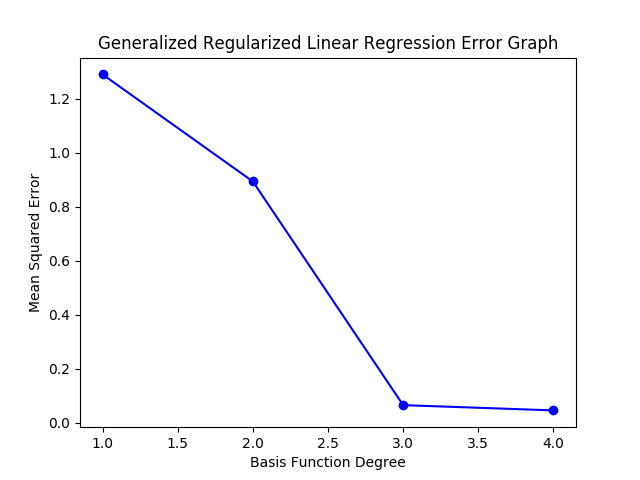
\includegraphics[width=0.6\textwidth]{3a_degree_vs_error.png}
            \caption{Regularized Generalized Linear Regression - Error vs Basis function degree}
            \label{fig:rglg_err_v_deg}
        \end{figure}

        Similarly, Figure \ref{fig:rglg_time_v_deg} shows the variation of time required for the computation as a function of the maximum basis function degree. The experiments might not be very indicative of the complexity increase, due to the low amount of time the computation actually takes, but the computation seems to be increasing monotonically for increased maximum degree of basis functions. This could be attributed to the increase of the size of the weights that need to be computed, because each `n' degree basis function is a subset of any `m' degree basis function $\forall m > n$

        \begin{figure}[ht]
            \centering
            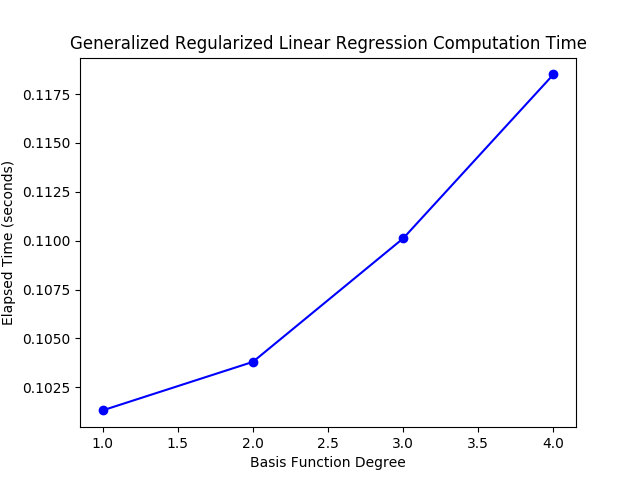
\includegraphics[width=0.6\textwidth]{3a_degree_vs_time.png}
            \caption{Regularized Generalized Linear Regression - Time vs Basis function degree}
            \label{fig:rglg_time_v_deg}
        \end{figure}

        The code for Regularized Generalized Linear Regression is present in the directory `regularized-generalized-linear-regression' of the code archive submitted.

    % subsection regularized_generalized_linear_regression (end)

    \subsection{Bayesian Generalized Linear Regression} % (fold)
    \label{sub:bayesian_generalized_linear_regression}
    
        Figure \ref{fig:bglg_err_v_deg} shows how the model error varies with respect to the maximum degree of basis functions. The best performing basis function in terms of error minimization is the one with degree 4.

        \begin{figure}[ht]
            \centering
            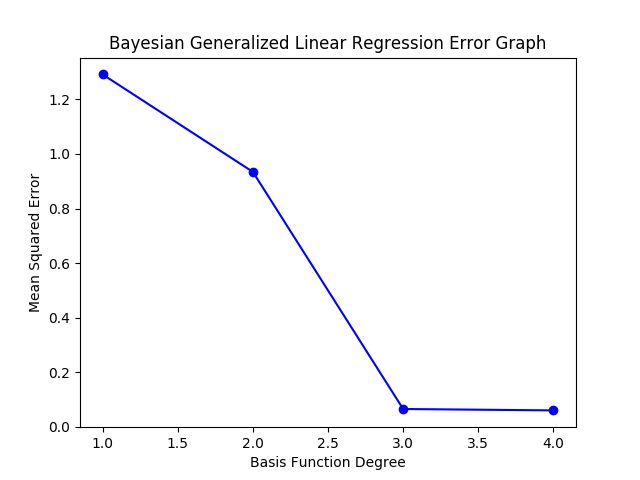
\includegraphics[width=0.6\textwidth]{3b_degree_vs_error.png}
            \caption{Bayesian Generalized Linear Regression - Error vs Basis function degree}
            \label{fig:bglg_err_v_deg}
        \end{figure}

        Figure \ref{fig:bglg_time_v_deg} shows the variation of time required for the computation as a function of the maximum basis function degree. The patterns in the function are similar to those detected for Regularized Generalized Linear Regression. 

        \begin{figure}[ht]
            \centering
            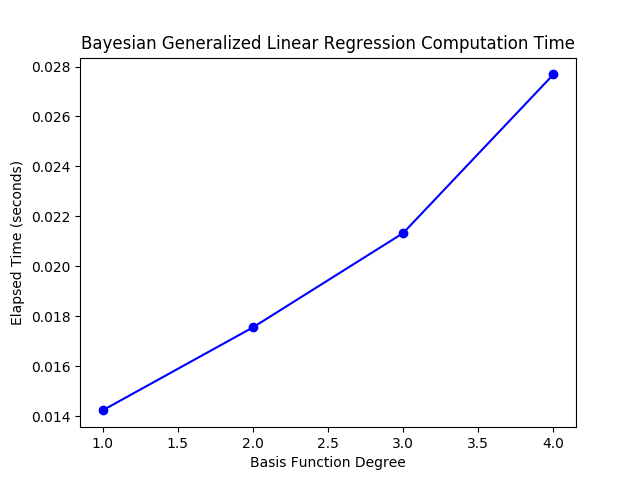
\includegraphics[width=0.6\textwidth]{3b_degree_vs_time.png}
            \caption{Bayesian Generalized Linear Regression - Time vs Basis function degree}
            \label{fig:bglg_time_v_deg}
        \end{figure}

        The code for Bayesian Generalized Linear Regression is present in the directory `bayesian-generalized-linear-regression' of the code archive submitted.

        \subsubsection*{Regularized generalized linear regression vs. Bayesian generalized linear regression} % (fold)
        \label{ssub:regularized_generalized_linear_regression_vs_bayesian_generalized_linear_regression}

            The generalized version of linear regression allows a mapping into a higher dimensional feature space which can be utilized to perform linear regression to predict underlying functions are are non-linear. This approach is common to both Regularized generalized linear regression and Bayesian generalized linear regression.

            The difference between the two models is that Bayesian linear regression models the weight parameter as a Gaussian distribution. This leads to modeling the Bayesian linear objective's target variable as a conjugate distribution. This is because both the prior and likelihood probability distributions are Gaussian, which implicity models the target variable distribution as a Gaussian, too. This different from regularized generalized linear regression, as for the latter, we simply obtain the solution by minimizing a convex optimization objective, whereas for bayesian generalized linear regression, we iteratively minimize the search space for the ideal weights by using the computed posterior of each data-point as a prior for the next expression, thus minimizing the risk of overfitting better that simple generalized linear models.
        
        % subsubsection regularized_generalized_linear_regression_vs_bayesian_generalized_linear_regression (end)
    
    % subsection bayesian_generalized_linear_regression (end)

    \subsection{Gaussian Process Regression} % (fold)
    \label{sub:gaussian_process_regression}
    
    % subsection gaussian_process_regression (end)

% section non_linear_regression_techniques (end)


\end{document}
